\section{Introduction}

The first wall of a fusion reactor is a two-material system. A plasma-facing
material meets the plasma, withstanding extreme heat flux, particle bombardment,
and neutron irradiation, while a structural alloy behind it carries the mechanical
load. Tungsten leads as the plasma-facing material for its high melting point, low
sputtering yield, and good thermal conductivity, but it is brittle and unsuited to a load-bearing role~\cite{tungstenPFMreview2023}, whereas reduced-activation
ferritic-martensitic steels such as EUROFER97 serve as the structural material
with favorable activation but limited high-temperature
capability~\cite{lindau2005eurofer,RAFMreview2017}. Both must also resist
irradiation damage and remain acceptably activated through operation and
decommissioning~\cite{zinkle2000operating,bloom2007critical}. No single material
satisfies the surface and structural requirements simultaneously, so the first
wall is necessarily built from a plasma-facing material and a structural material
that must somehow be joined into one component.

Joining these materials is a central difficulty. Tungsten and steel differ
markedly in thermal expansion (coefficients of roughly \(4.4\) and
\(12.7 \times 10^{-6}\)~K\(^{-1}\)), so an abrupt joint concentrates large thermal
stresses, and direct tungsten-iron contact forms brittle intermetallics,
principally Fe\(_2\)W and Fe\(_7\)W\(_6\), that embrittle the
joint~\cite{fgmWsteelCGS2022,karim2024wire}. A functionally graded alloy, whose
composition varies continuously from a tungsten-rich plasma-facing terminal to a
structural terminal, can spread the expansion mismatch over a graded region rather
than a single boundary~\cite{fgmWEurofer2015}; such gradients are now
practically realizable, with additive manufacturing routes such as directed
energy deposition able to vary the feed composition layer by
layer~\cite{karim2024wire}. Grading alone, however, does not avoid the intermetallics, since iron and
tungsten still meet across the gradient. The remedy is to keep the transition
a single body-centered cubic (BCC) solid solution at every step, so the path
never enters the composition ranges where the brittle phases are
stable~\cite{fgmWsteelInterlayerBCC2023}. This choice replaces the structural
terminal itself. Rather than grading toward a steel such as EUROFER97, the
gradient terminates in a vanadium-rich structural alloy, low in activation
and reachable from tungsten through a continuous BCC path, so that iron and
tungsten no longer meet along the transition. Finding such a path by
inspection is difficult, since the constraints interact across the
composition space, and existing realizations rely on a few hand-selected
interlayers chosen one composition at a
time~\cite{fgmWsteelInterlayerBCC2023}. Here we instead search the entire
feasible composition space for the graded path directly, so the single-phase
transition is designed rather than assembled from discrete steps.

Designing such a path is a constrained search. The role-specific demands are
divided between the terminals, the plasma-facing side taking the
high-temperature requirement and the structural side the ductility
requirement, but the requirements shared by the whole wall, low activation, a
stable single-phase structure, and adequate thermal conductivity, must be met
by both terminals and every intermediate step alike. Multicomponent
refractory alloys offer wide freedom to balance these
demands~\cite{HEAnuclear2021,Senkov2010}, and high-throughput screening under
multiple simultaneous property constraints has proven effective for
navigating refractory alloy spaces of this kind, combining CALPHAD
thermodynamics with physics-based strength and ductility models to reduce
vast composition spaces to actionable candidate
sets~\cite{vela2023data,HTcalphad2022}. The scale remains demanding, however,
as an eleven-element system on a \(5\)~at.\% grid already spans tens of
millions of compositions, far more than can be tested, and among the
criteria, neutron-induced activation is especially consequential, since
transmutation governs decay heat, dose rates, maintenance, and waste
burden~\cite{RAFMreview2017}, motivating low-activation, radiation-tolerant
elements~\cite{HEAnuclear2021,ElAtwani2019Radiation}.

The First Wall Loading and Activation Response Engine (FLARE) makes the
activation criteria tractable at this scale
\textcolor{red}{\cite{flare}}. Rather than running a full inventory
calculation for every candidate, FLARE precomputes the activation response of
each pure element under a fixed irradiation and decay scenario, so that the
response of any alloy follows as a composition-weighted combination of these
elemental contributions, compared against references such as pure tungsten
and EUROFER97. Because every response is such a weighted combination, the
activation criteria are linear in composition, and the compositions
satisfying all of them form a convex region bounded by the constraint
hyperplanes. Linear programming describes this region directly, so the
feasible space is obtained without evaluating the candidates one by one, and
it is used here as the screening step rather than as the object of the work.

The feasible space is the starting point for the design. Within it, high-throughput
thermodynamic and mechanical evaluation identifies the compositions that are
single-phase, thermally conductive, and suited to the plasma-facing and structural
roles. Treating these compositions as nodes on a simplex lattice, with neighbors
connected by single-step composition changes, turns the design space into a graph
whose connected regions can be traversed~\cite{nimplex}. The two terminals are
located within the largest connected, single-phase region, and the graded path
between them is found as the shortest route through this graph along feasible
neighbors only, which yields the most gradual feasible transition, the fewest
single-step composition changes between terminals. The path is additionally
required to be monotonic in both design properties, with the solidus
temperature never increasing and the ductility never decreasing from the
plasma-facing terminal to the structural terminal, so that no interior layer
of the graded wall is hotter-melting than the layer in front of it or less
ductile than the layer behind it. The same connectivity that
defines the connected feasible regions also supplies the routes between
compositions, so the identification of the design region and the construction of
the graded path follow from a single graph. The path therefore stays single-phase
and activation-feasible at every step and never enters the ranges where brittle
intermetallics would form.

Path planning in composition space has an established lineage in the design of
compositionally graded alloys. Kirk et al.\ introduced a computational
methodology that plans gradient paths through high-dimensional composition
spaces while avoiding undesirable phase regions~\cite{kirk2018gradient}, an
approach subsequently realized experimentally in additively manufactured
gradients~\cite{eliseeva2019fgm}, and later extended the framework to produce
paths with monotonic property profiles, on the argument that a monotonic
gradient can be reshaped into nearly any spatial profile on the part by
controlling the deposition rate~\cite{kirk2021monotonic}. In that work
monotonicity is promoted through a penalized cost function whose weight must
be selected, and it is treated for a single property at a time, with extension
to multiple properties explicitly identified as future
work~\cite{kirk2021monotonic}. Graph representations of composition space
have also been extended, within the same design framework, to multi-terminal
graded structures~\cite{multiterminalCGA2024}, though without property
monotonicity. The graded
first wall poses a harder version of the problem: two properties with opposing
trends, a solidus that must only decrease and a ductility that must only
increase along the same path, with every intermediate composition
simultaneously subject to activation, phase-stability, and conductivity
constraints. To our knowledge, path planning under simultaneous monotonicity
in two opposing properties has not been reported; here it is enforced not
through a tuned penalty but as a hard constraint, by deleting every
property-violating transition from the graph before an exact shortest-path
search.

In this work we design a functionally graded alloy for the fusion first wall in
an eleven-element refractory system \ch{Cr-Fe-Hf-Mo-Nb-Re-Ta-Ti-V-W-Zr}. The
contribution is a doubly-monotonic, single-phase compositional path from a
tungsten-rich plasma-facing terminal to a vanadium-rich structural terminal
that remains activation-feasible throughout, avoiding the brittle
intermetallics that limit conventional tungsten-to-steel graded joints.
Activation screening referenced to tungsten and EUROFER97 defines the feasible
space; thermodynamic and mechanical evaluation reduces it to a connected
single-phase region governed by phase stability, thermal conductivity, solidus
temperature, and ductility; and graph-based path design connects the terminals
through it. To our knowledge, this is the first compositional gradient designed
under simultaneous monotonicity in two opposing properties. The resulting path achieves monotonicity at zero cost in path length,
passing exclusively through the small set of compositions that form the only
monotone gateway between the two categories, and the framework, summarized
in Figure~\ref{fig:overview}, applies generally to graded-alloy design
governed by composition-linear screening models.



\begin{figure*}[!t]
  \centering
  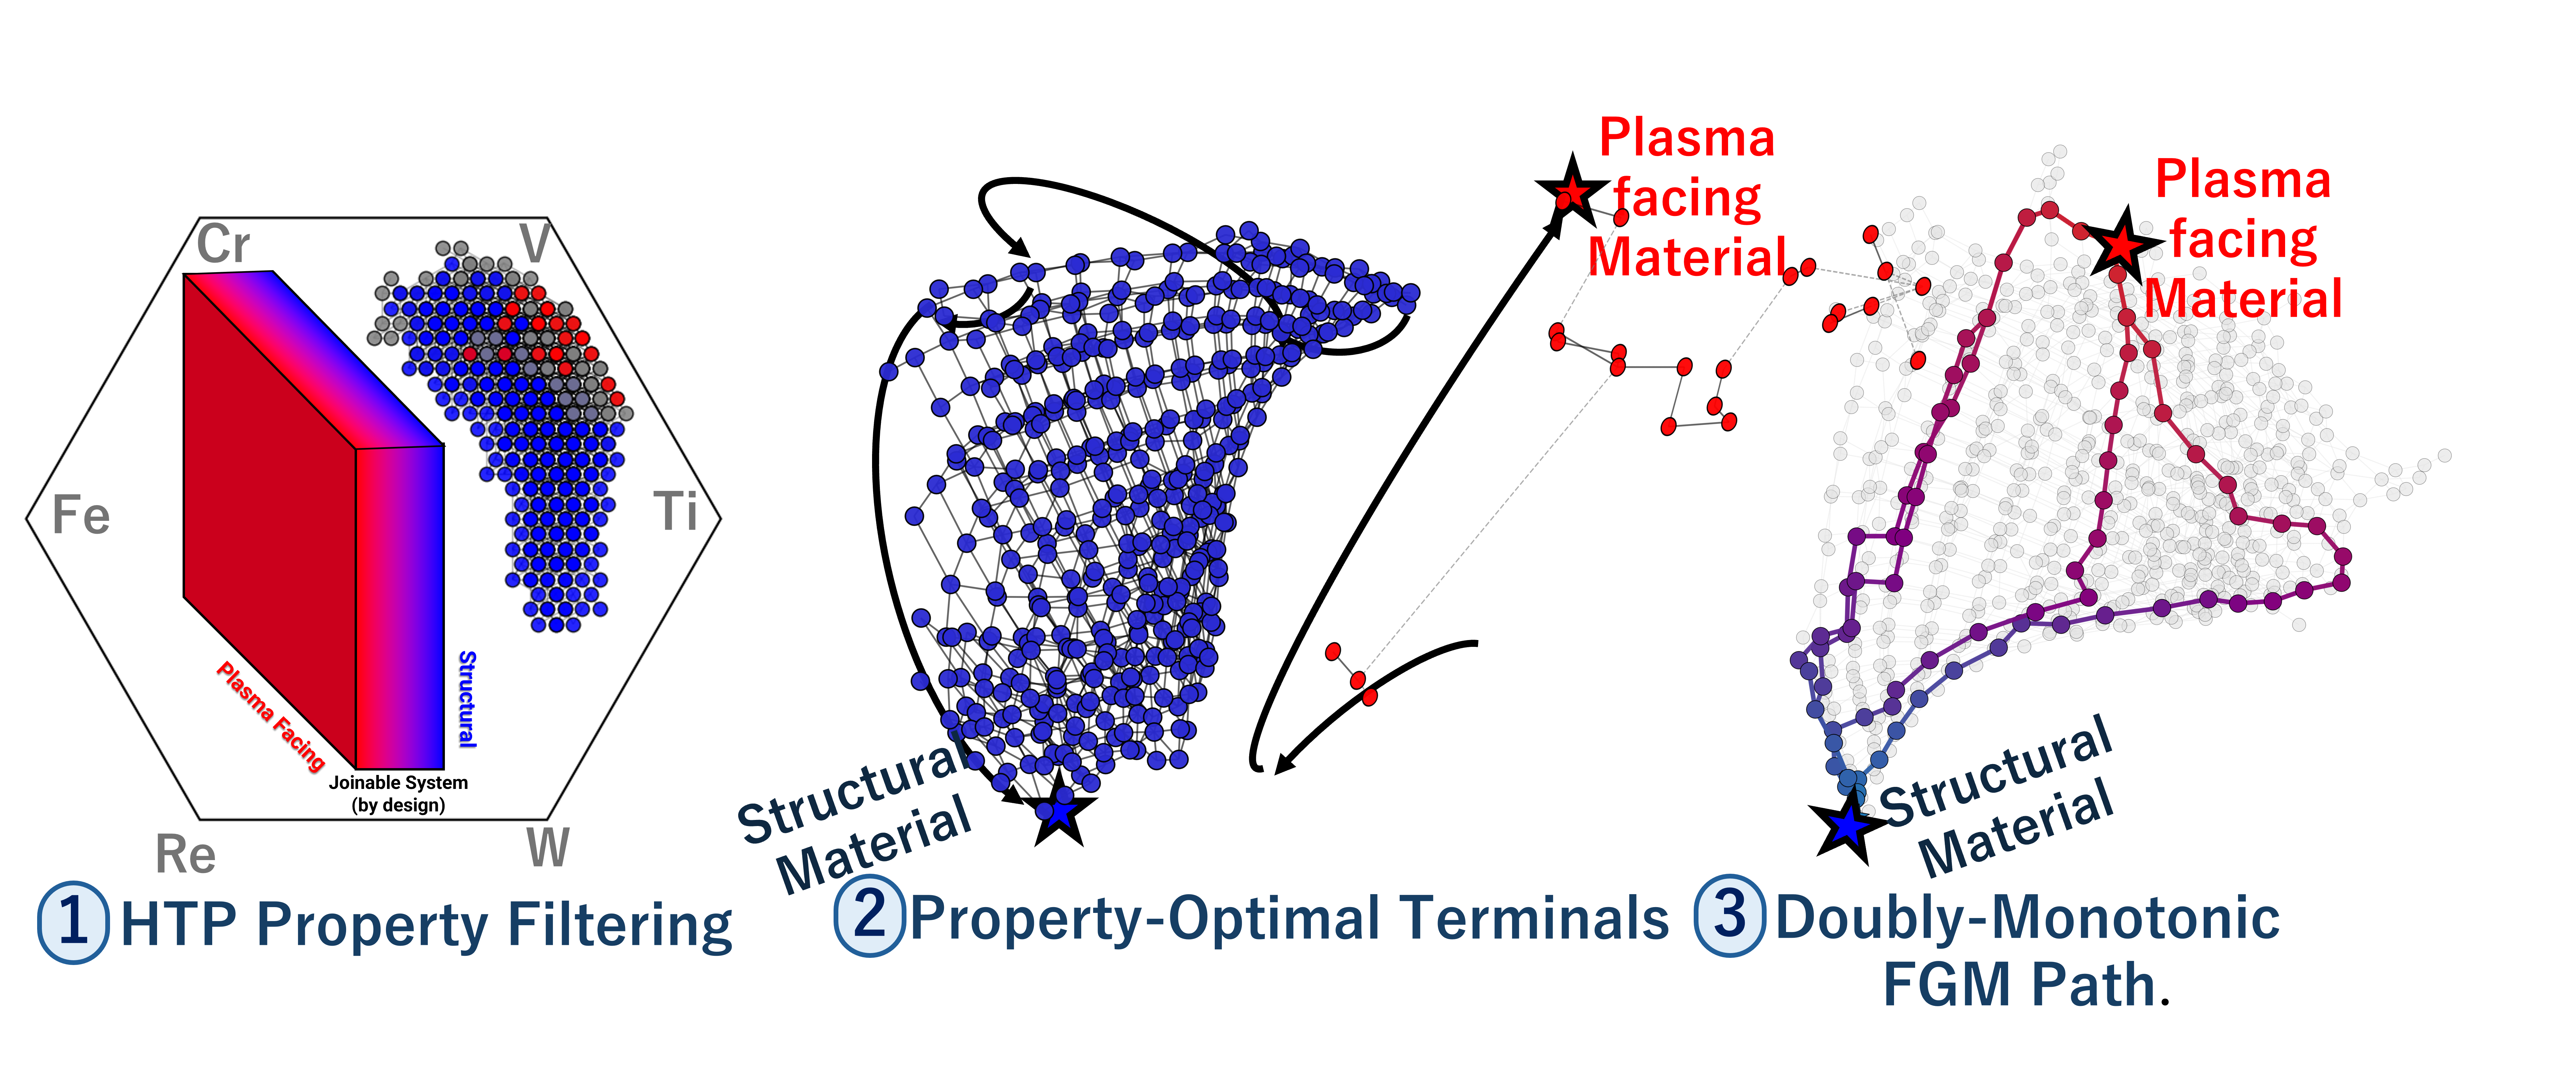
\includegraphics[width=0.9\textwidth]{figures/FGM-SCHEMATIC.png}
 \caption{Overview of the design workflow: property filtering of the
activation-feasible composition space, selection of the plasma-facing and
structural terminals, and doubly-monotonic graded-path design.}
  \label{fig:overview}
\end{figure*}